\documentclass[10pt,a4paper]{article}
\usepackage{amsmath,amssymb}
\usepackage{graphicx}
\usepackage{booktabs}
\usepackage{geometry}
\geometry{margin=0.62in}
\usepackage{xcolor}
\usepackage{enumitem}
\usepackage{hyperref}
\hypersetup{colorlinks=true, urlcolor=cyan}
\pagestyle{empty}
\setlength{\parskip}{2pt}\setlength{\parindent}{0pt}

\begin{document}

{\Large \textbf{Aims 1 and 2 update: measuring the language component in multilingual LLMs}}\\[1mm]
{\small Waiz Khan (\texttt{wkhan12@jh.edu}); one-page dashboard; 5-page
findings brief and full technical report available. July 2026.}

\vspace{1.2mm}\hrule\vspace{1.4mm}

\begin{center}
\footnotesize\textbf{17 models (0.6B--9B) $\cdot$ 122--128 languages $\cdot$
31 pre-registered predictions, 21 passed $\cdot$ 4/4 blind prospective test
$\cdot$ 7 self-caught errors, all documented}
\end{center}
\vspace{-1.5mm}

\vspace{1.6mm}
\begin{minipage}[t]{0.585\textwidth}
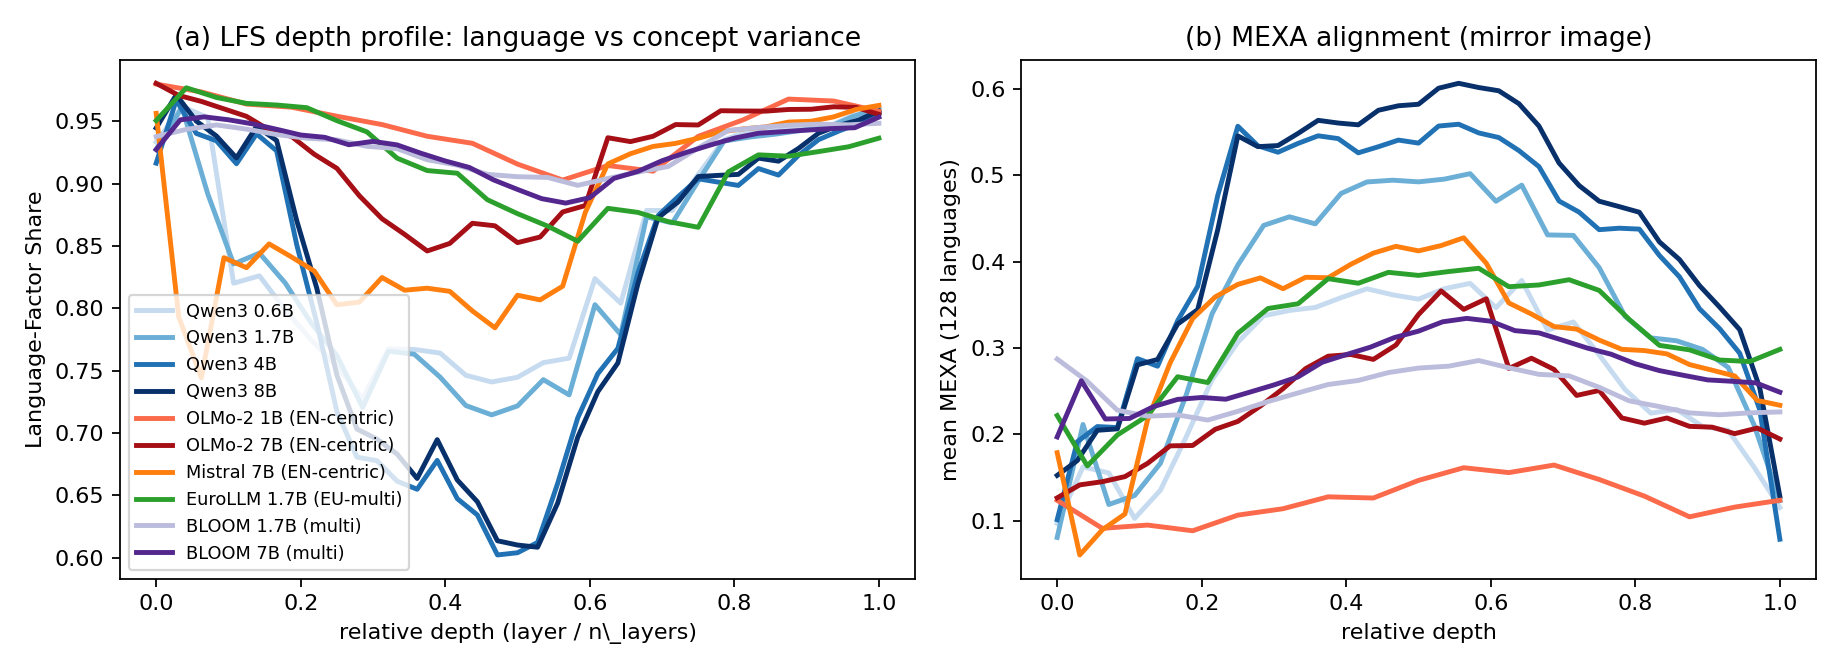
\includegraphics[width=\textwidth]{figs/fig1_lfs_depth_profile.png}
{\scriptsize The \textbf{Language-Factor Share} (LFS): per-layer variance share
owned by language identity; a direct operational measure of \S3.1.1's
``how strong the language component is.''}
\end{minipage}\hfill
\begin{minipage}[t]{0.385\textwidth}
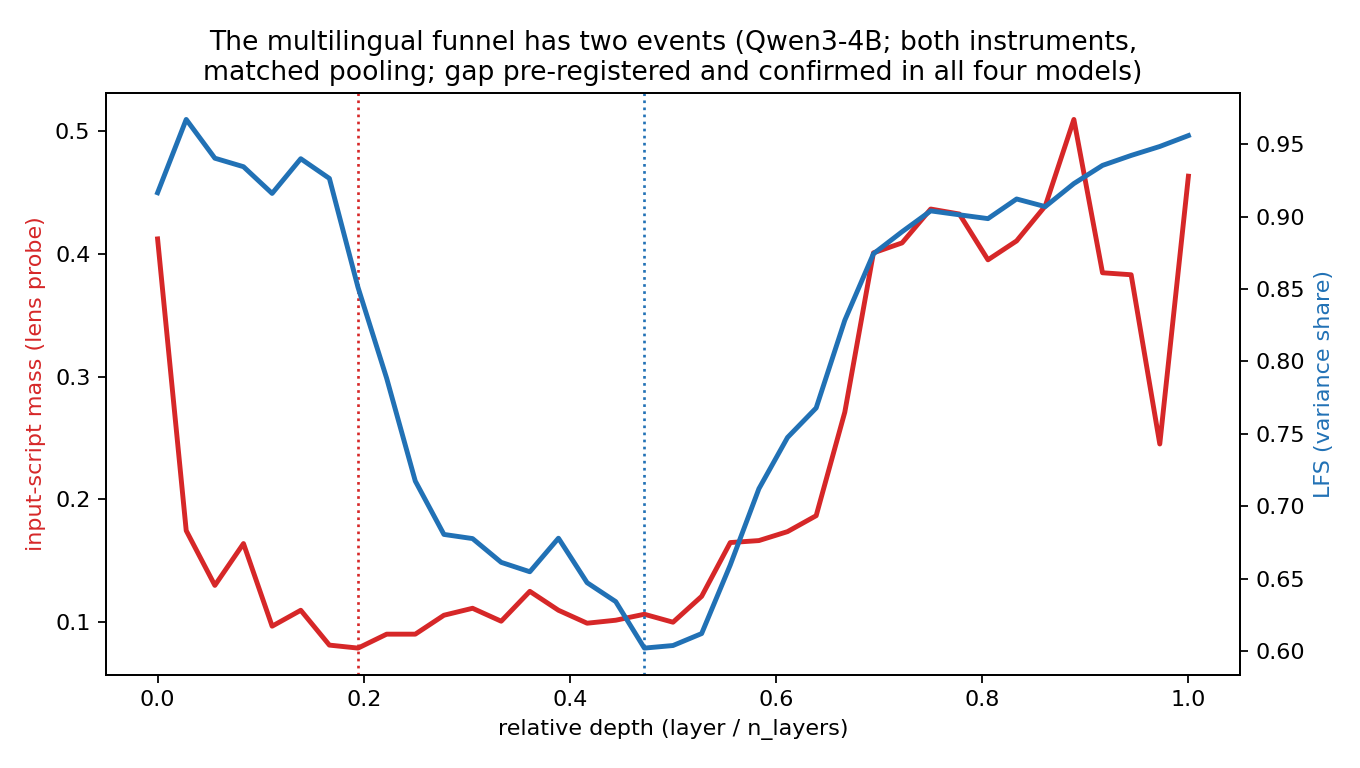
\includegraphics[width=\textwidth]{figs/fig12_twoevents.png}
{\scriptsize The depth profile has \textbf{two events}: script abandoned early,
concepts converge mid; pre-registered, confirmed twice.}
\end{minipage}

\vspace{1.6mm}
{\normalsize\textbf{Ten findings}}\\[-3.2mm]
\begin{enumerate}[leftmargin=1.35em, itemsep=0.35mm, parsep=0pt, topsep=1mm]
\small
\item \textbf{\S3.1.1, measured:} shared-space depth dips in the middle layers and recovers, and varies
$0.04$--$0.34$ across models; a measurable, model-dependent quantity.
\item \textbf{Two-event depth profile:} surface script drops out early ($\sim$0.1
depth); meanings converge mid ($\sim$0.4). New structure, twice confirmed.
\item \textbf{Family separates more than scale:} between-family spread at fixed size dwarfs
within-family scaling slope; Qwen3-1.7B out-converges every other lab's 7B.
\item \textbf{Coverage $\neq$ convergence:} BLOOM (deliberately 46-language)
has the flattest concept space; its alignment lives in the embedding layer (surface form, not meaning), invariant from 1.7B to 7B.
\item \textbf{``Thinks in English'' is resource-graded and fading:} a
multilingual latent factor out-predicts English for 113 to 124 of 127 languages by model (124 for most)
($+0.08$ after confound correction); English's best-donor share falls
45$\to$25/127 as Qwen3 scales.
\item \textbf{The mean hides the tail:} mid-resource languages pass averages
while worst-decile sentences sit at retrieval failure; the tail is
\emph{semantic} (anaphora, culturally-bound vocabulary), not entity noise; \textbf{Alignment-at-Risk (AaR)} reports it.
\item \textbf{Confounder-adjusted validity:} on this grid, $\sim$40--60\% of the raw
metric$\leftrightarrow$performance correlation is observables (data size,
family, script, fertility); the surviving range is $\rho \approx 0.19$--$0.31$ (the July figure of about 0.59 on a benchmark-capable subset is withdrawn: not reproducible from any stored artifact). The tail measure AaR adds the tail visibility that is its job; MEXA is reported alongside for reference and is not ranked against it.
\item \textbf{Predicts behavior beyond observables (observationally):}
alignment at the LFS-identified layer predicts generation-time cross-lingual
context use at confounder-adjusted $\rho = 0.67$ (language-clustered CI $[0.55, 0.77]$;
mismatched-context controlled). Tested under intervention, the association
does not transfer: see the Aim-2 entry below.
\item \textbf{Prospective test, 4/4 blind:} two untouched families (SmolLM2,
Falcon3) matched their predicted recipe class; held-out validity exceeded the
development CI; preregistered prediction P4 (a tail-measure-versus-MEXA difference on the benchmark-capable subgroup) passed on one held-out model ($\Delta = +0.14$, CI $[+0.03, +0.26]$) and is not used as a ranking.
\item \textbf{Aim-2 study, 28 conditions $\times$ three seeds, four objective
families:} every condition fails its frozen criteria. The objective \S3.2.2
specifies degenerates by \textbf{89\%}, and \emph{neither LFS nor MEXA detects
it}: both are scale-invariant, and the scale-collapsed condition posts among the highest
retrieval and best tail alignment in the study. The decomposition separates
collapsed from sound by $20\times$; the ratio divides that out.
\textbf{Report the component profile, not the share.} A collapse guard is
necessary and structurally insufficient (bounded hinge, unbounded objective).
\emph{LFS is a measurement, not a training target.}
\end{enumerate}

\vspace{0.8mm}\hrule\vspace{1.2mm}
{\small \textbf{How it was validated:} every main claim pre-registered or
adjusted for observables; failures printed beside successes; code and
frozen protocols release-ready. \quad \textbf{Ask:} 30 minutes; (i) the
constrained Aim-2 objective the study implies, (ii) venue + remaining
pre-submission items, (iii) coordination with adjacent work in the group.}

\end{document}
